\begin{figure}
  \centering
  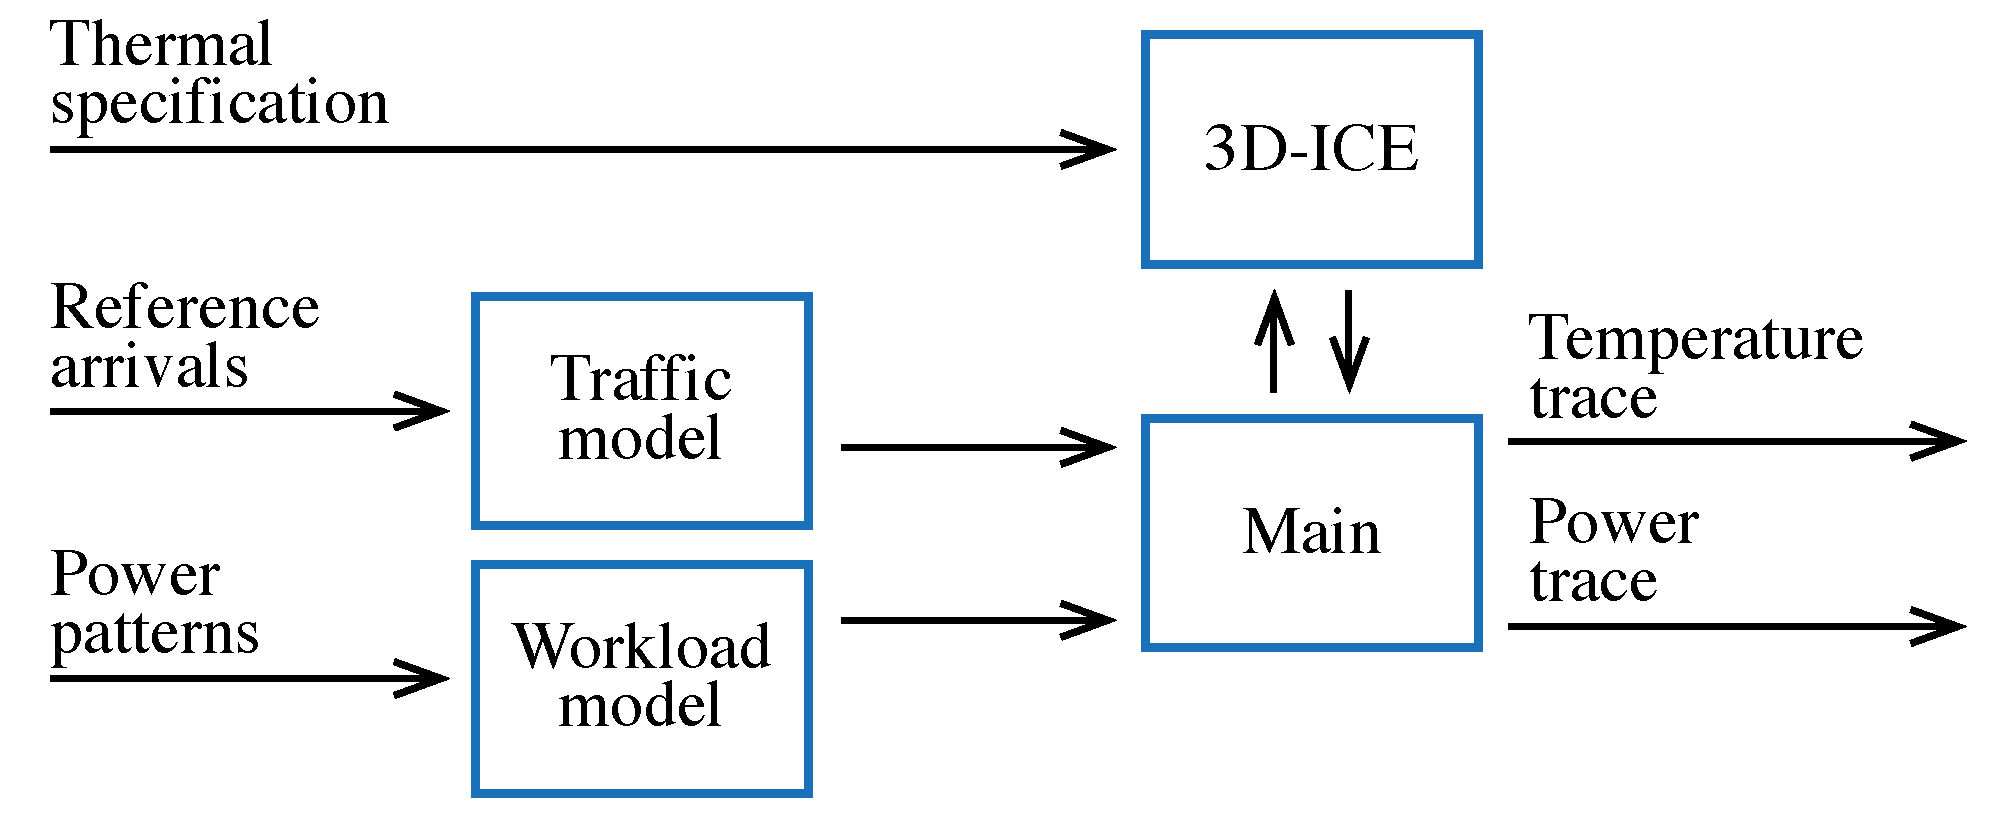
\includegraphics[width=1.0\columnwidth]{include/assets/figures/streamer.pdf}
  \caption{The streaming infrastructure.}
  \flab{streamer}
\end{figure}

The Streamer tool corresponds to the data-synthesis stage. It is responsible for
synthesizing power and temperature data using reference data as a material for
the synthesis. In \fref{methodology}, it corresponds to the rightmost box
labeled ``Streamer.'' The structure of the tool is illustrated in
\fref{streamer}.

Given a traffic pattern and a set of workload patterns, Streamer proceeds as
follows. The traffic pattern is processed as it is described in \sref{traffic},
which results in an adequately configured multifractal wavelet model
\cite{riedi1999}. The model is then used to generate a stream of arrival times.
The arrival times are substantiated using the workload patterns, which is
explained in \sref{workload}. The result is a stream of jobs. In
\fref{streamer}, the whole above operation takes place in the box labeled ``Job
model.'' The rest follows \sref{composition}. Namely, the job stream is first
handled by the user's resource manager, which resides in the box labeled
``Main.'' As jobs are being scheduled, the power profile of the system is being
progressively constructed. The power profile is piped into a temperature
simulator (to be discussed), which delivers a temperature profile. Finally, the
synthesized power and temperature profiles are made available to the manager.
They can also be saved on disk, in which case, similar to reference data, the
output is an SQLite database.

Let us now elaborate on the temperature simulation that Streamer undertakes. It
is based on the well-known thermal \sc{RC} model. We construct a thermal \sc{RC}
circuit for the platform at hand and then use it for analyzing the thermal
behavior of the system. The analysis boils down to solving a system of
differential equations. In our case, the solution is based on a solver
leveraging exponential integrators \cite{ukhov2014}. The construction of thermal
circuits is delegated to either HotSpot \cite{skadron2004} or \sc{3D-ICE}
\cite{sridhar2010} (see \fref{streamer}) depending on the user's preferences.

To summarize, Recorder captures workload patterns, and Streamer produces streams
of power and temperature data. Both closely follow the methodology described in
\sref{methodology}.
